\documentclass[10pt, a4paper]{article}  % Любой документ начинается с такой строки! В ней мы выбираем 
\author{Голованова Лиза}
\usepackage{amsmath,amsfonts,amssymb,amsthm,mathtools}  % Тут мы подключаем пакеты для математики!
\usepackage{graphicx}
\graphicspath{{Pics/}}
\DeclareGraphicsExtensions{.pdf,.png,.jpg}
\usepackage{fontspec}         % пакет для подгрузки шрифтов
\setmainfont{Roboto}          % задаёт основной шрифт документа

\usepackage{unicode-math}     % пакет для установки математического шрифта
\setmathfont{Asana Math}      % шрифт для математики

\usepackage{polyglossia}      % Пакет, который позволяет подгружать русские буквы
\setdefaultlanguage{russian}  % Основной язык документа
\setotherlanguage{english}    % Второстепенный язык документа
\usepackage{ tipa }
\usepackage{mathrsfs}

\begin{document} 
\section*{Задание 1}
\subsection*{10 благородных истин обо мне}

\begin{enumerate}
\item $\heartsuit$ $\curlywedge$ ю $\delta$ $\curlywedge$ ю $\heartsuit$ сложности;
\item Училась в одной из топ 10 школ Оксфорда;
\item Умею дружить и выбирать себе друзей;
\item Люблю книги о деятельных людях;
\item Не понимаю и не люблю артхаус;
\item Большàя часть моего багажа бытовых и культурных знаний изъята из 10 заграничных стран; 
\item Люблю все предметы, которые хорошо преподаются; 
\item Самый бунтарский поступок в моей жизни связан с осуществлением одной из моих мечт;
\item Терпеть не могу праздники, выходные и каникулы;
\item Отношусь к людям, которым вполне достаточно самого лучшего.
\end{enumerate}

\section*{Задание 2}

\begin{figure}[h]
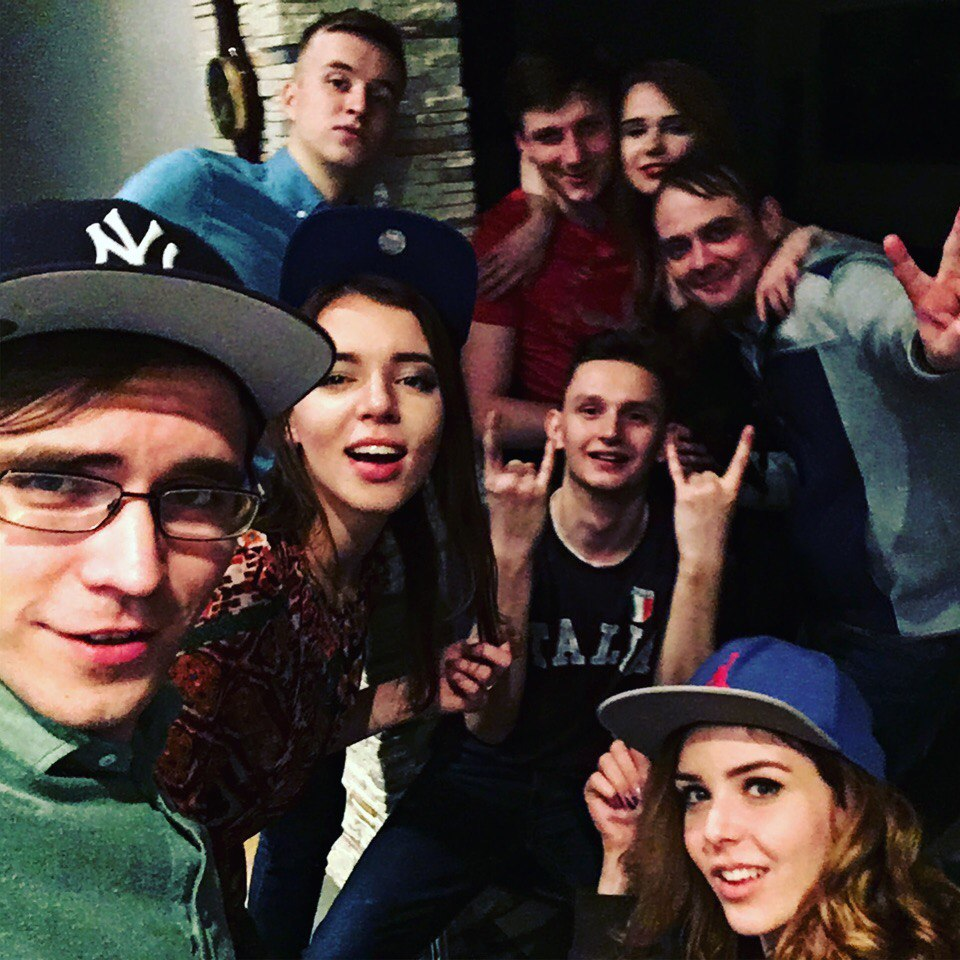
\includegraphics[scale=0.25]{image}
\caption{На этой фотке есть я!}
\end{figure}

\section*{Задание 3}
\subsection*{Мои любимые формулы}

 \begin{align}
 \lim_{n\to 0}(1+x)^{1+x}=\lim_{\alpha\to\infty}(1+\dfrac{1}{\alpha})^{\alpha}=e \tag{\ae}\label{aster1}
 \end{align}
 \begin{align}
\int\limits_{\--\infty}^\infty\mathrm{e}^{-x^2}\,\mathrm{d}x\int\limits_{\--\infty}^\infty\mathrm{e}^{-y^2}\,\mathrm{d}y=\uppi \tag{\ae\ae}\label{aster2}
 \end{align}
 \begin{align}
\mathrm{e}(\hat{\theta_n})=\dfrac{1}{n*\textsci(\theta)*\mathcal{D}(\hat{\theta_n})} \tag{\ae\ae\ae}\label{aster3}
 \end{align}
 \begin{align}
Var(s)=Var(E(s|r))+E(Var(s|r))  \tag{\ae\ae\ae\ae}\label{aster4}
 \end{align}
 \begin{align}
\begin{vmatrix} 
a_1 & b_1 & c_1 \\ 
a_2 & b_2 & c_2\\ 
a_3 & b_3 & c_3 \end{vmatrix}=a_1*b_2*c_3−a_1*b_3*c_2+b_1*c_2*a_3 − b_1*c_3*a_2+ c_1*a_2* b_3−c_1* a_3* b_2  \tag{\ae\ae\ae\ae\ae}\label{aster5}
 \end{align} 
 
\subsection*{Ненавистная формула}
 \begin{equation*}
 \sum_{n=2}^{N} \dfrac{1}{n^p} < \int_1^N \dfrac{\mathrm{d}x}{x^p}=\int_1^N x^{-p}\mathrm{d}x=\left.\dfrac{x^{1-p}}{1-p}\right|_1^N =$$
$$ = \dfrac{N^{1-p}-1}{1-p}=\dfrac{1-N^{1-p}}{p-1}<\dfrac{1}{p-1} 
 \end{equation*} 
 
%\tag{\ae\ae\ae\ae\ae\ae}\label{aster6}

\section*{Задание 4}
\subsection*{Почему я люблю и ненавижу формулы}

Формулы ~\ref{aster1} и ~\ref{aster2} мне по душе, потому что я не люблю знать короткий ответ на то, что решать у меня получается не очень хорошо. Формула ~\ref{aster3} напоминает мне о прекрасных временах, когда я разозлилась на свои результаты по учебе и начала "очаровывать" Палыча. (Он так сам сказал, да-да!). Формула ~\ref{aster4} почему-то очень хорошо спрятана от людей, даже в Интернете не обсуждается. Она дает мне чувство преимущества, когда я ее использую, в то время, как остальные перешептываются:"Откуда она это взяла???" Формулу ~\ref{aster5} просто невозможно не любить!
 А формулу ненавистную формулу невозможно любить, потому что:
\begin{enumerate}
\item Она была дана на лекциях Попова
\item Я не понимаю ряды 
\item Я даже не могу на нее сослаться(((
\end{enumerate}


\end{document}